\ifx\HO\undefined
\documentclass{beamer}
\usepackage{animate}
%\usepackage{CJKutf8}
%\AtBeginDvi{\input{zhwinfonts}}
\usepackage{amsthm}
\usepackage{pgfpages}
\usepackage{beamerthemesplit}
\usetheme[headheight=0pt,footheight=0pt]{boxes}
\else
\documentclass[9pt,handout]{beamer}
%\usepackage{animate}
%\usepackage{CJKutf8}
%\AtBeginDvi{\input{zhwinfonts}}
\usepackage{amsthm}
\usepackage{pgfpages}
\usepackage{beamerthemesplit}
\usetheme[headheight=0pt,footheight=0pt]{boxes}
\pgfpagesuselayout{4 on 1}[a4paper,border shrink=5mm,landscape]
\fi

\beamertemplatenavigationsymbolsempty

\usepackage{tikz}
\input{../macros/macros}
%\newtheorem*{theorem*}{Theorem}
%\newtheorem*{lemma*}{Lemma}
%\newtheorem*{proposition*}{Proposition}
%\newtheorem*{corollary*}{Corollary}
%\theoremstyle{definition}
%\newtheorem*{remark*}{Remark}
%\newtheorem*{definition*}{Definition}
%\newtheorem*{example*}{Example}
%\newtheorem*{method*}{Method}
%\newtheorem*{fact*}{Fact}
% Exercises are numbered separately
%\newtheorem*{exercise*}{Exercise}

% \newenvironment{theorem*}[1]{{\Large\BLUE{Theorem #1:}}}{}
% \newenvironment{lemma*}[1]{{\Large\BLUE{Lemma #1:}}}{}
% \newenvironment{proposition*}[1]{{\Large\BLUE{Proposition #1:}}}{}
% \newenvironment{corollary*}[1]{{\Large\BLUE{Corollary #1:}}}{}
% \newenvironment{remark*}[1]{{\Large\BLUE{Remark #1:}}}{}
% \newenvironment{definition*}[1]{{\Large\BLUE{Definition #1:}}}{}
% \newenvironment{example*}[1]{{\Large\BLUE{Example #1:}}}{}
% \newenvironment{method*}[1]{{\Large\BLUE{Method #1:}}}{}
% \newenvironment{fact*}[1]{{\Large\BLUE{Fact #1:}}}{}

\newenvironment{theorem*}[1]{{\Large\BLUE{Theorem:}}}{}
\newenvironment{lemma*}[1]{{\Large\BLUE{Lemma:}}}{}
\newenvironment{proposition*}[1]{{\Large\BLUE{Proposition:}}}{}
\newenvironment{corollary*}[1]{{\Large\BLUE{Corollary:}}}{}
\newenvironment{remark*}[1]{{\Large\BLUE{Remark:}}}{}
\newenvironment{definition*}[1]{{\Large\BLUE{Definition:}}}{}
\newenvironment{example*}[1]{{\Large\BLUE{Example:}}}{}
\newenvironment{method*}[1]{{\Large\BLUE{Method:}}}{}
\newenvironment{fact*}[1]{{\Large\BLUE{Fact:}}}{}

\newenvironment{eg}{{\Large\OLG{Example:}} }{}

\newcommand{\startproof}{{\Large\BLUE{Proof:}\;\;}}
\title{Introduction}
\author{}

\begin{document}

\begin{frame}[t]
 \frametitle{Normal form for the Bessel equation}
 \vspace{-6ex}
 \[ y''+Py'+Qy=0 \qquad
    m = \exp(-\half\int P\,dx) \qquad
    R =Q-\half P'-\tfrac{1}{4}P^2 \qquad
 \] \[
    y = mz \qquad
    z''+Rz=0
 \]

 \reminderbar
 
 \uc<2->{Consider again the Bessel equation $x^2y''+xy'+(x^2-n^2)y=0$.}\\
 \uc<3->{We can divide by $x^2$ to get $y''+x^{-1}y'+(1-n^2x^{-2})y=0$.}\\
 \uc<4->{This is $y''+Py'+Qy=0$, where $P=x^{-1}$ and $Q=1-n^2x^{-2}$.}\\
 \uc<5->{We now have
 \begin{align*}
  \uc<5->{m} &\uc<5->{= \exp(-\half\int P\,dx)}\uc<6->{ = \exp(-\half\ln(x)) = x^{-1/2}} \\
  \uc<7->{R} &\uc<7->{= Q - \half P' - \tfrac{1}{4}P^2} 
              \uc<8->{= 1-n^2x^{-2}+\half x^{-2}-\tfrac{1}{4}x^{-2}}
              \uc<9->{= 1 + \frac{1-4n^2}{4x^2}}
 \end{align*}}

 \uc<10->{Conclusion: the solutions for $x^2y''+xy'+(x^2-n^2)y=0$ have the 
  form $y=x^{-1/2}z$, where $z''+\left(1+\frac{1-4n^2}{4x^2}\right)z=0$.}  

 \uc<11->{For large $x$, this is approximately $z''+z=0$, so $z$ is like
  $A\cos(x+\phi)$, so $y$ is like $Ax^{-1/2}\cos(x+\phi)$.} 
\end{frame}

\begin{frame}[t]
 \frametitle{Normal form for the Bessel equation}
  \[ \begin{array}{cc}
     \includegraphics[scale=0.16]{images/besselj0.pdf} &
     \includegraphics[scale=0.16]{images/besselj1.pdf} \\
     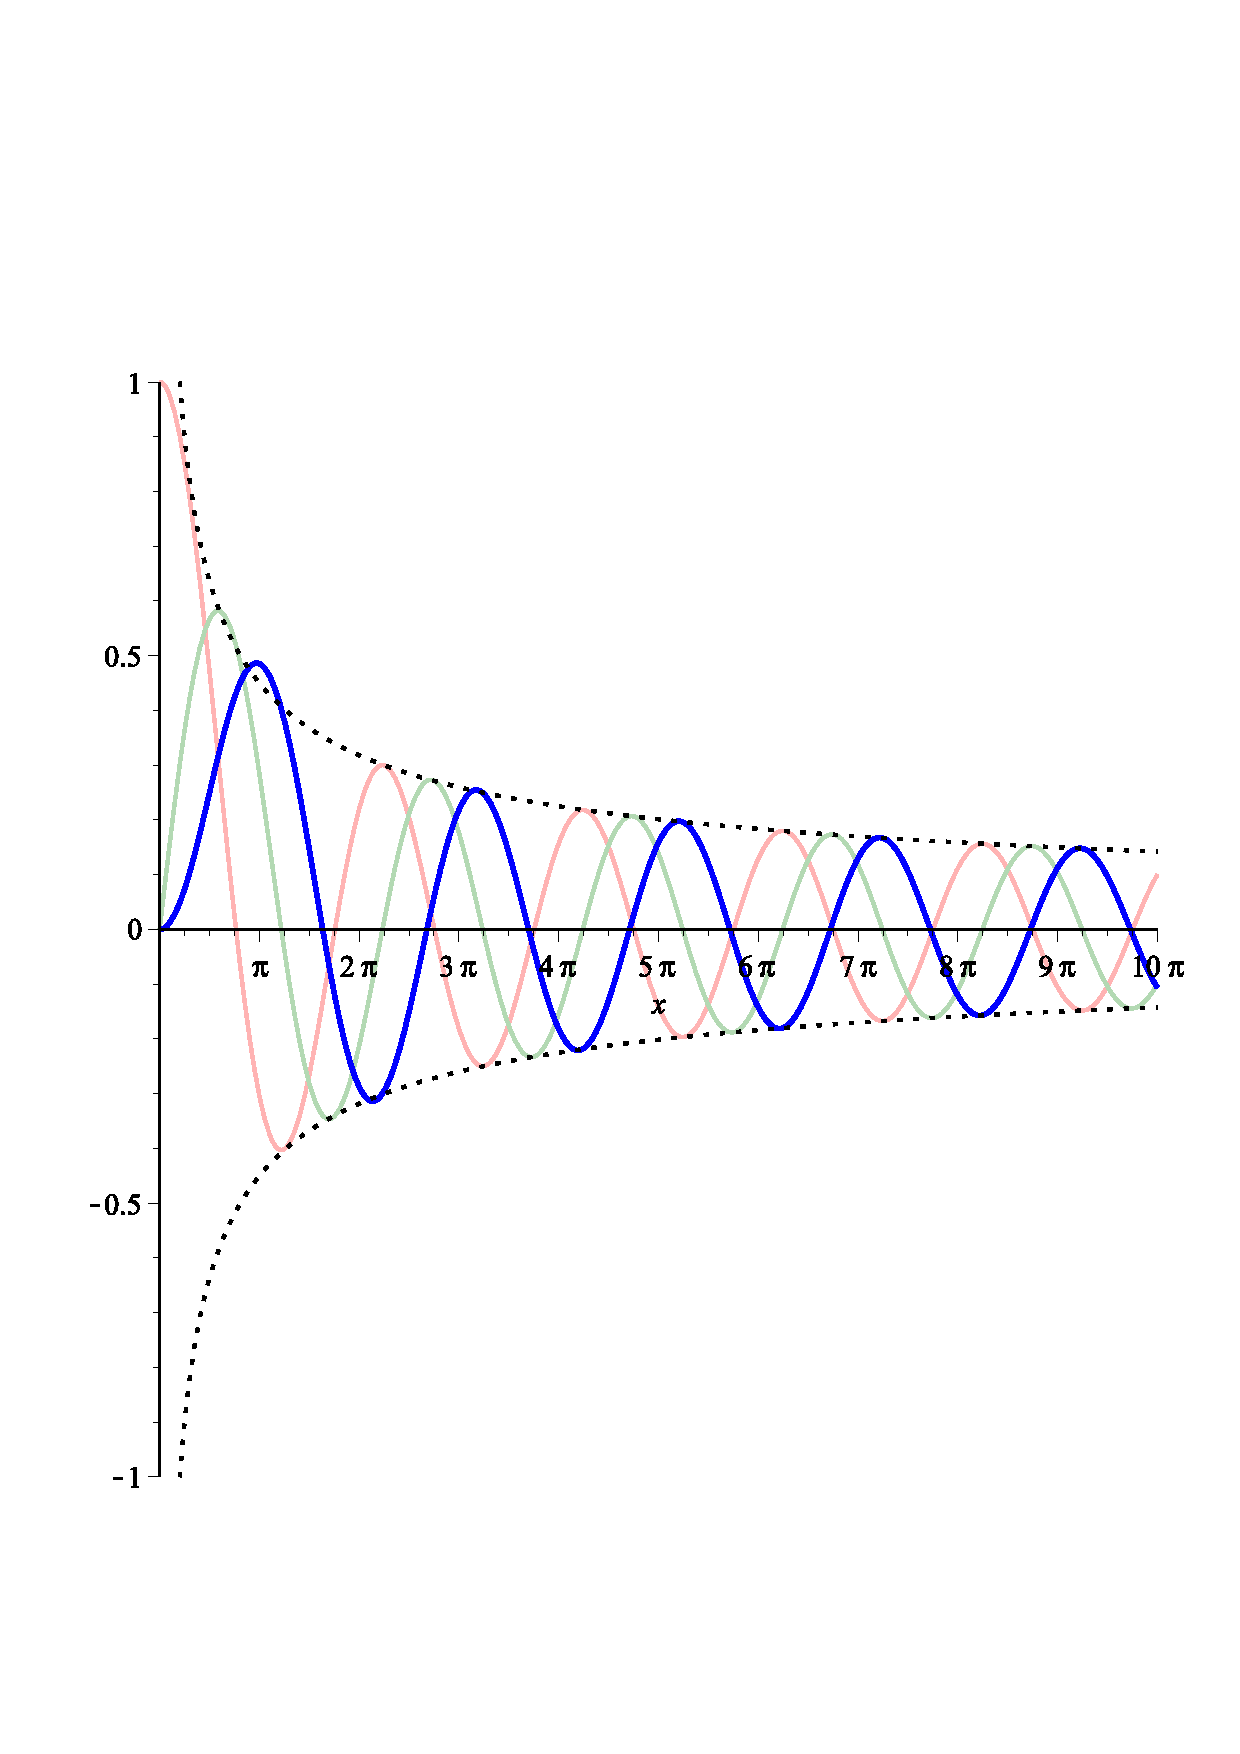
\includegraphics[scale=0.16]{images/besselj2.pdf} &
     \includegraphics[scale=0.16]{images/besselj3.pdf} 
  \end{array} \]
  For large $x$, this is approximately $z''+z=0$, so $z$ is like
  $A\cos(x+\phi)$, so $y$ is like $Ax^{-1/2}\cos(x+\phi)$
\end{frame}

\end{document}




%%%%%%%%%%%%%%%%%%%%%%%%%%%%%%%%%%%%%%%%%%%%%%%%%%%%%%%%%%%%%%%%%%%%%%


